\documentclass[border=4pt]{standalone}

\usepackage[T1]{fontenc}
\usepackage[utf8]{inputenc}
\usepackage{amsmath}
\usepackage{xcolor}
\usepackage{tikz}
\usetikzlibrary{positioning, fit, calc, arrows.meta, backgrounds}

\begin{document}
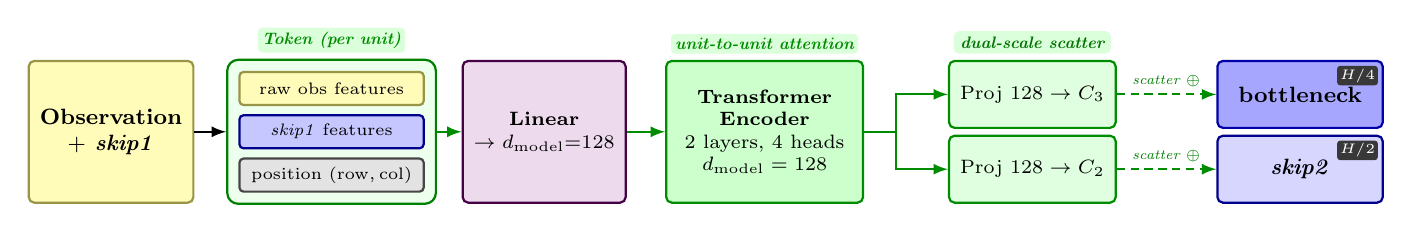
\begin{tikzpicture}[
    >=latex,
    blk/.style={draw, rounded corners=2pt, align=center, thick, inner sep=4pt, font=\scriptsize},
    ent/.style={blk, fill=green!20, draw=green!55!black, minimum width=2.5cm, minimum height=1.8cm},
    linblk/.style={blk, fill=violet!14, draw=violet!55!black, minimum width=1.5cm, minimum height=1.8cm},
    io/.style={blk, fill=yellow!28, draw=yellow!55!black, minimum width=1.7cm, minimum height=1.8cm, font=\footnotesize\bfseries},
    proj/.style={blk, fill=green!12, draw=green!55!black, minimum width=2.0cm, minimum height=0.85cm},
    bot/.style={blk, fill=blue!35, draw=blue!65!black, minimum width=2.1cm, minimum height=0.85cm, font=\footnotesize\bfseries},
    spatial/.style={blk, fill=blue!16, draw=blue!55!black, minimum width=2.1cm, minimum height=0.85cm, font=\footnotesize\bfseries},
    tokencomp/.style={draw, rounded corners=1.5pt, align=center, thick, text width=2.2cm, minimum height=0.42cm, font=\fontsize{6.5pt}{8pt}\selectfont, inner sep=2pt},
    rawtok/.style={tokencomp, fill=yellow!28, draw=yellow!55!black},
    skiptok/.style={tokencomp, fill=blue!22, draw=blue!55!black},
    postok/.style={tokencomp, fill=gray!22, draw=gray!55!black},
    flow/.style={->, thick},
    entflow/.style={->, thick, green!55!black},
    scflow/.style={->, thick, densely dashed, green!55!black},
    grouplbl/.style={font=\fontsize{6pt}{7pt}\selectfont\bfseries\itshape, rounded corners=1.5pt, inner sep=1.5pt, fill=white},
    sublbl/.style={font=\scriptsize\itshape, text=gray!55!black, fill=white, inner sep=1.5pt},
    % Scatter +/oplus label: even smaller (5pt)
    scatlbl/.style={font=\fontsize{2pt}{2.5pt}\selectfont\itshape, text=green!50!black, fill=white, inner sep=0.2pt},
    scatterlbl/.style={font=\fontsize{6pt}{7pt}\selectfont\bfseries\itshape, text=green!45!black, fill=green!14, rounded corners=2pt, inner sep=2pt, align=center, minimum width=2.0cm},
    pill/.style={fill=black!78, text=white, rounded corners=1pt, inner sep=1pt, font=\fontsize{5pt}{6pt}\selectfont\bfseries, anchor=north east},
]

% ─── Stage 1: Input ───
\node[io] at (0, 0) (grid) {Observation\\$+$ \emph{skip1}};

% ─── Stage 2: Token (3 same-size components) ───
\node[rawtok]  at (2.8, 0.55)  (raw)   {raw obs features};
\node[skiptok] at (2.8, 0.0)   (skip)  {\emph{skip1} features};
\node[postok]  at (2.8, -0.55) (pos)   {position $(\mathrm{row}, \mathrm{col})$};

% Token group box (background)
\begin{scope}[on background layer]
    \node[fill=green!7, rounded corners=4pt, draw=green!50!black, thick, inner sep=4pt,
          fit=(raw)(skip)(pos)] (tokgroup) {};
\end{scope}
\node[grouplbl, text=green!55!black, fill=green!14, anchor=south]
    at ([yshift=2pt]tokgroup.north) {Token (per unit)};

% ─── Stage 3: Linear ───
\node[linblk] at (5.5, 0) (linear) {{\bfseries Linear}\\$\to d_{\mathrm{model}}{=}128$};

% ─── Stage 4: Transformer encoder ───
\node[ent] at (8.3, 0) (tr) {{\bfseries Transformer}\\{\bfseries Encoder}\\2 layers, 4 heads\\$d_{\mathrm{model}}=128$};
\node[grouplbl, text=green!55!black, fill=green!14, anchor=south]
    at ([yshift=2pt]tr.north) {unit-to-unit attention};

% ─── Stage 5: Two projection blocks (lowered slightly so tops align with tokgroup/tr tops) ───
\node[proj] at (11.7, 0.475)  (proj_bot)  {Proj $128 \to C_3$};
\node[proj] at (11.7, -0.475) (proj_s2)   {Proj $128 \to C_2$};

% ─── Dual-scale scatter (south-anchored at same y as other banners) ───
\node[scatterlbl, anchor=south] at ([yshift=2pt]proj_bot.north) {dual-scale scatter};

% ─── Stage 6: Scatter targets (aligned with projs) ───
\node[bot]     at (15.1, 0.475)  (bot_target) {bottleneck};
\node[spatial] at (15.1, -0.475) (s2_target)  {\emph{skip2}};

\node[pill] at ([shift={(-2pt,-2pt)}]bot_target.north east) {$H/4$};
\node[pill] at ([shift={(-2pt,-2pt)}]s2_target.north east)  {$H/2$};

% ─── Flows ───
\draw[flow]    (grid.east)     -- (tokgroup.west);
\draw[entflow] (tokgroup.east) -- (linear.west);
\draw[entflow] (linear.east)   -- (tr.west);

\coordinate (forkBase) at ($(tr.east) + (0.4, 0)$);
\draw[entflow] (tr.east) -- (forkBase) |- (proj_bot.west);
\draw[entflow] (forkBase) |- (proj_s2.west);

% Scatter arrows: label ABOVE the line, smaller font
\draw[scflow] (proj_bot.east) -- node[scatlbl, midway, above, yshift=2pt] {scatter $\oplus$} (bot_target.west);
\draw[scflow] (proj_s2.east)  -- node[scatlbl, midway, above, yshift=2pt] {scatter $\oplus$} (s2_target.west);

\end{tikzpicture}
\end{document}
